\documentclass[a4paper,11pt]{article} % fonte 11 points, papier a4

\usepackage[english]{babel} % language options
%\usepackage{textcomp}

\usepackage[utf8]{inputenc}   % character coding
\usepackage{amsmath}	% utilisation de gather
\usepackage{amssymb}    % sets symbols
\usepackage{siunitx}  % degree symbol and other units
\usepackage{numprint} % number formatting
\npdecimalsign{.}

%\usepackage[top=2.5cm, bottom=2.5cm, left=3.0cm, right=3.0cm]{geometry} % page geometry
\usepackage[top=1.0in, bottom=1.0in, left=1in, right=1in]{geometry} % page geometry

\usepackage{graphicx}   % introduction de graphiques
\usepackage{float}
\graphicspath{{images/}{.}}
\DeclareGraphicsExtensions{.pdf, .eps,.png,.jpg}
\usepackage{subcaption}
\usepackage{epstopdf} % image eps
%\usepackage[font=scriptsize]{caption}
\usepackage[font=small]{caption}
\setlength{\belowcaptionskip}{-10pt}
\setlength{\abovecaptionskip}{5pt}
%\usepackage{pdfpages} 	% Permet d'inclure des pages pdf.
%\usepackage{amssymb} % R symbol : $\mathbb{R}$

%\usepackage{listings}
%\usepackage{enumerate}



\usepackage{fancyhdr}	% en tete de page
\renewcommand{\headrulewidth}{0pt}
\setlength{\headheight}{15pt}
\fancypagestyle{plain}{%
  \fancyhf{}% Clear header/footer
  \fancyhead[L]{\color{gray}Ruslan Aydarkhanov and Florian Borse}% Right header
  \fancyfoot[C]{\color{gray}\thepage}% Right header
}
\pagestyle{plain}
%\pagestyle{empty}
%\pagestyle{headings}
%\addtolength{\textwidth}{1cm} %modifier les marges
%\addtolength{\hoffset}{-1cm}
%\addtolength{\textwidth}{2cm} 

% Sections
\usepackage{titlesec}
\titleformat{\section}{\large\bfseries}{Exercise \thesection.}{.35em}{}
%\renewcommand\thesubsection{(\alph{subsection})}
\titleformat{\subsection}[runin]{\itshape}{\thesubsection}{.35em}{}

% Hyper
%\usepackage[table,usenames,dvipsnames]{xcolor}
%\usepackage{hyperref} % Required for adding links   and customizing them
%\definecolor{linkcolour}{rgb}{0,0.2,0.6} % Link color
%\hypersetup{colorlinks,breaklinks,urlcolor=linkcolour,linkcolor=linkcolour} % Set link colors throughout the document


%%%%
% TODO PACKAGE
% Commands:
% - \missingfigure{Make a sketch of the structure of a trebuchet.}
% - \todo[inline,color=blue!20]{Put different methods until now + papers method}%
%\usepackage[colorinlistoftodos,disable]{todonotes} % Disable TODO
\usepackage[colorinlistoftodos]{todonotes} % Enable TODO
\newcommand{\todob}[1]{\todo[color=blue!20]{#1}}
\newcommand{\todobl}[1]{\todo[inline,color=blue!20]{#1}}
%%%%

%\setcounter
%###################
%% Début du document
%###################
\begin{document}

\begin{center}
    \bfseries\Large
    MiniProject:\\
    Modeling pacemaker neurons\\
    with the Hodgkin-Huxley model

\end{center}
%##################
%##################

\section{HH simulation}

\begin{figure}[H]
    \centering
    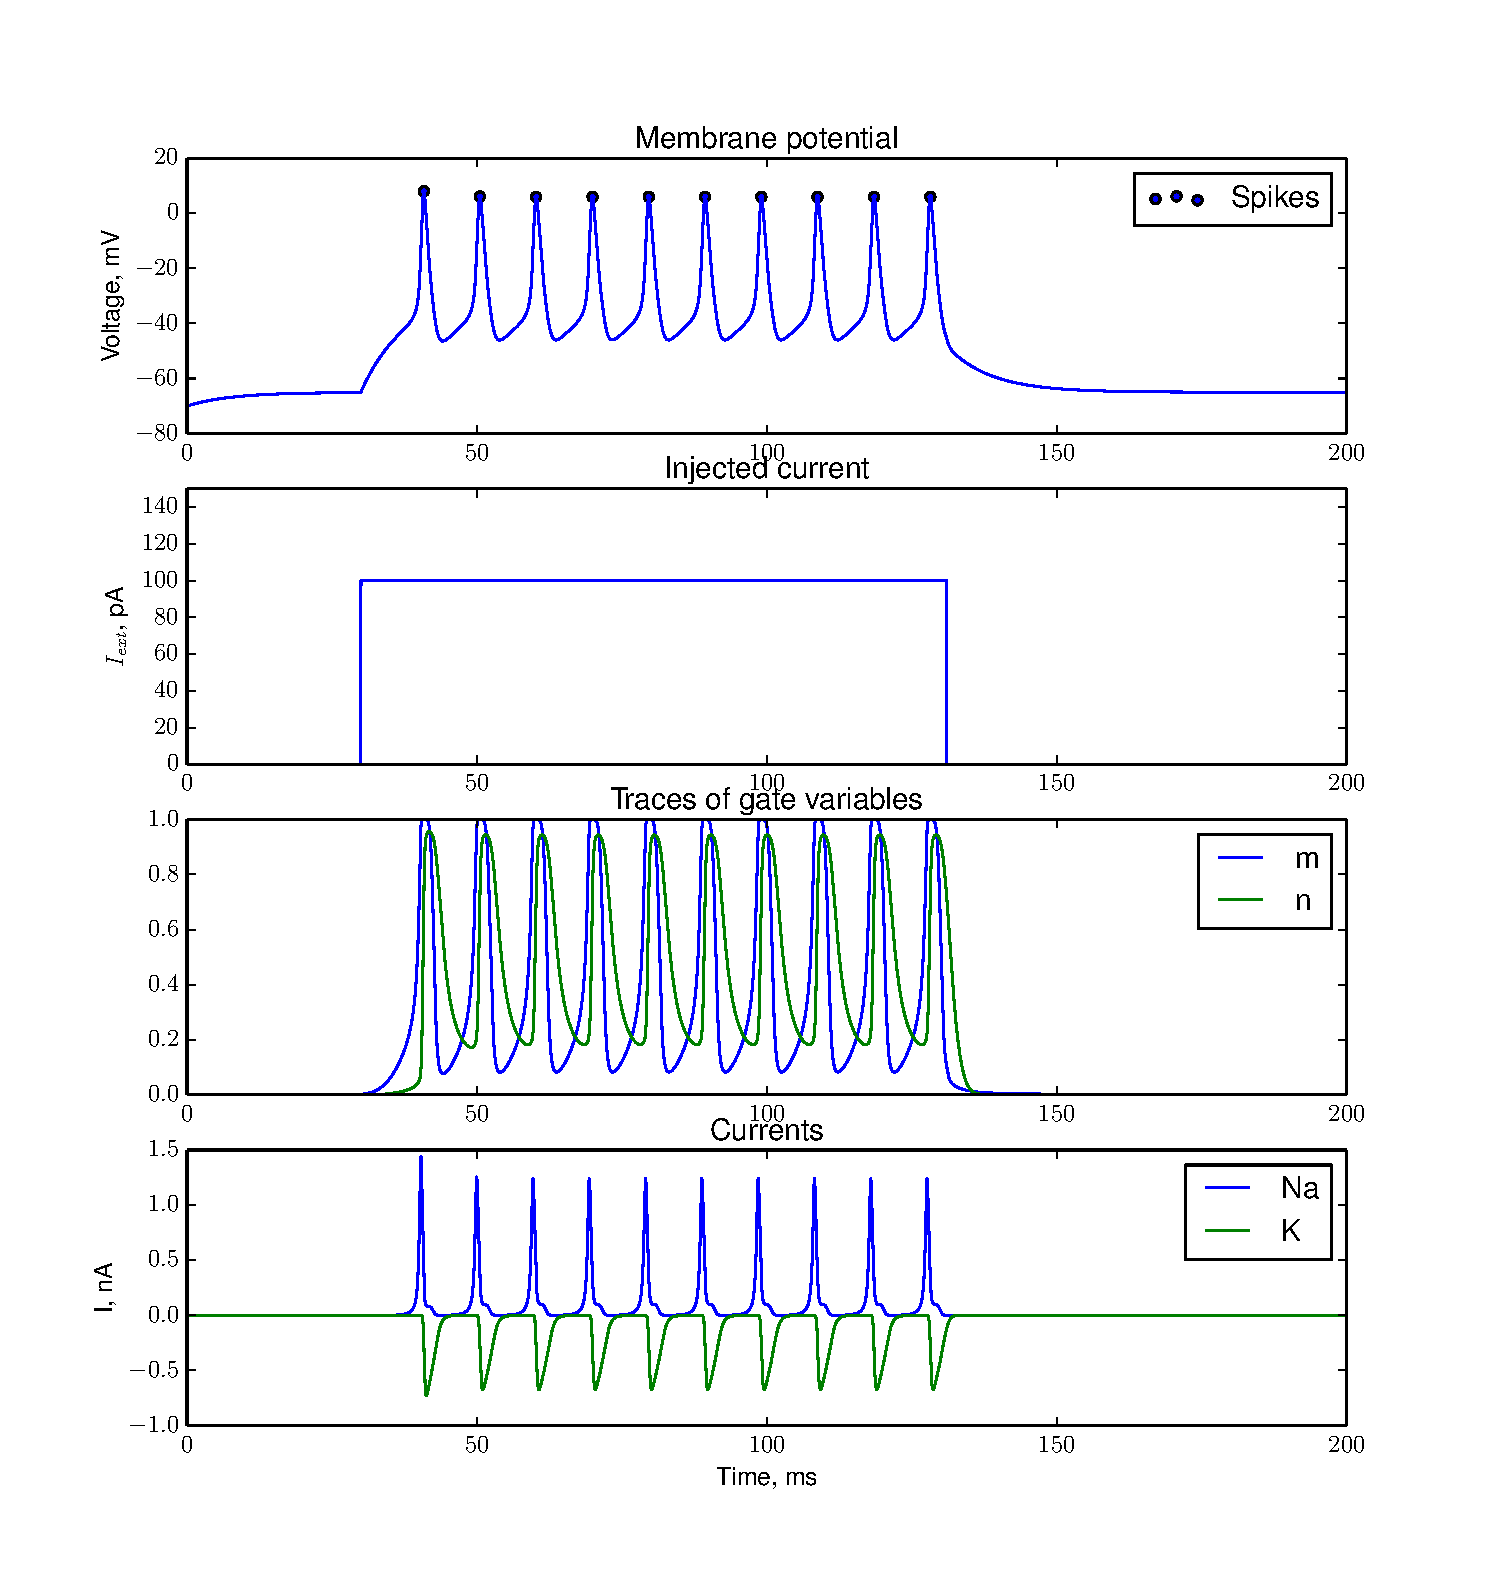
\includegraphics[width=\textwidth]{step_cur}
    \caption{Step current}
    \label{fig:step}
\end{figure}

\begin{figure}[H]
    \centering
    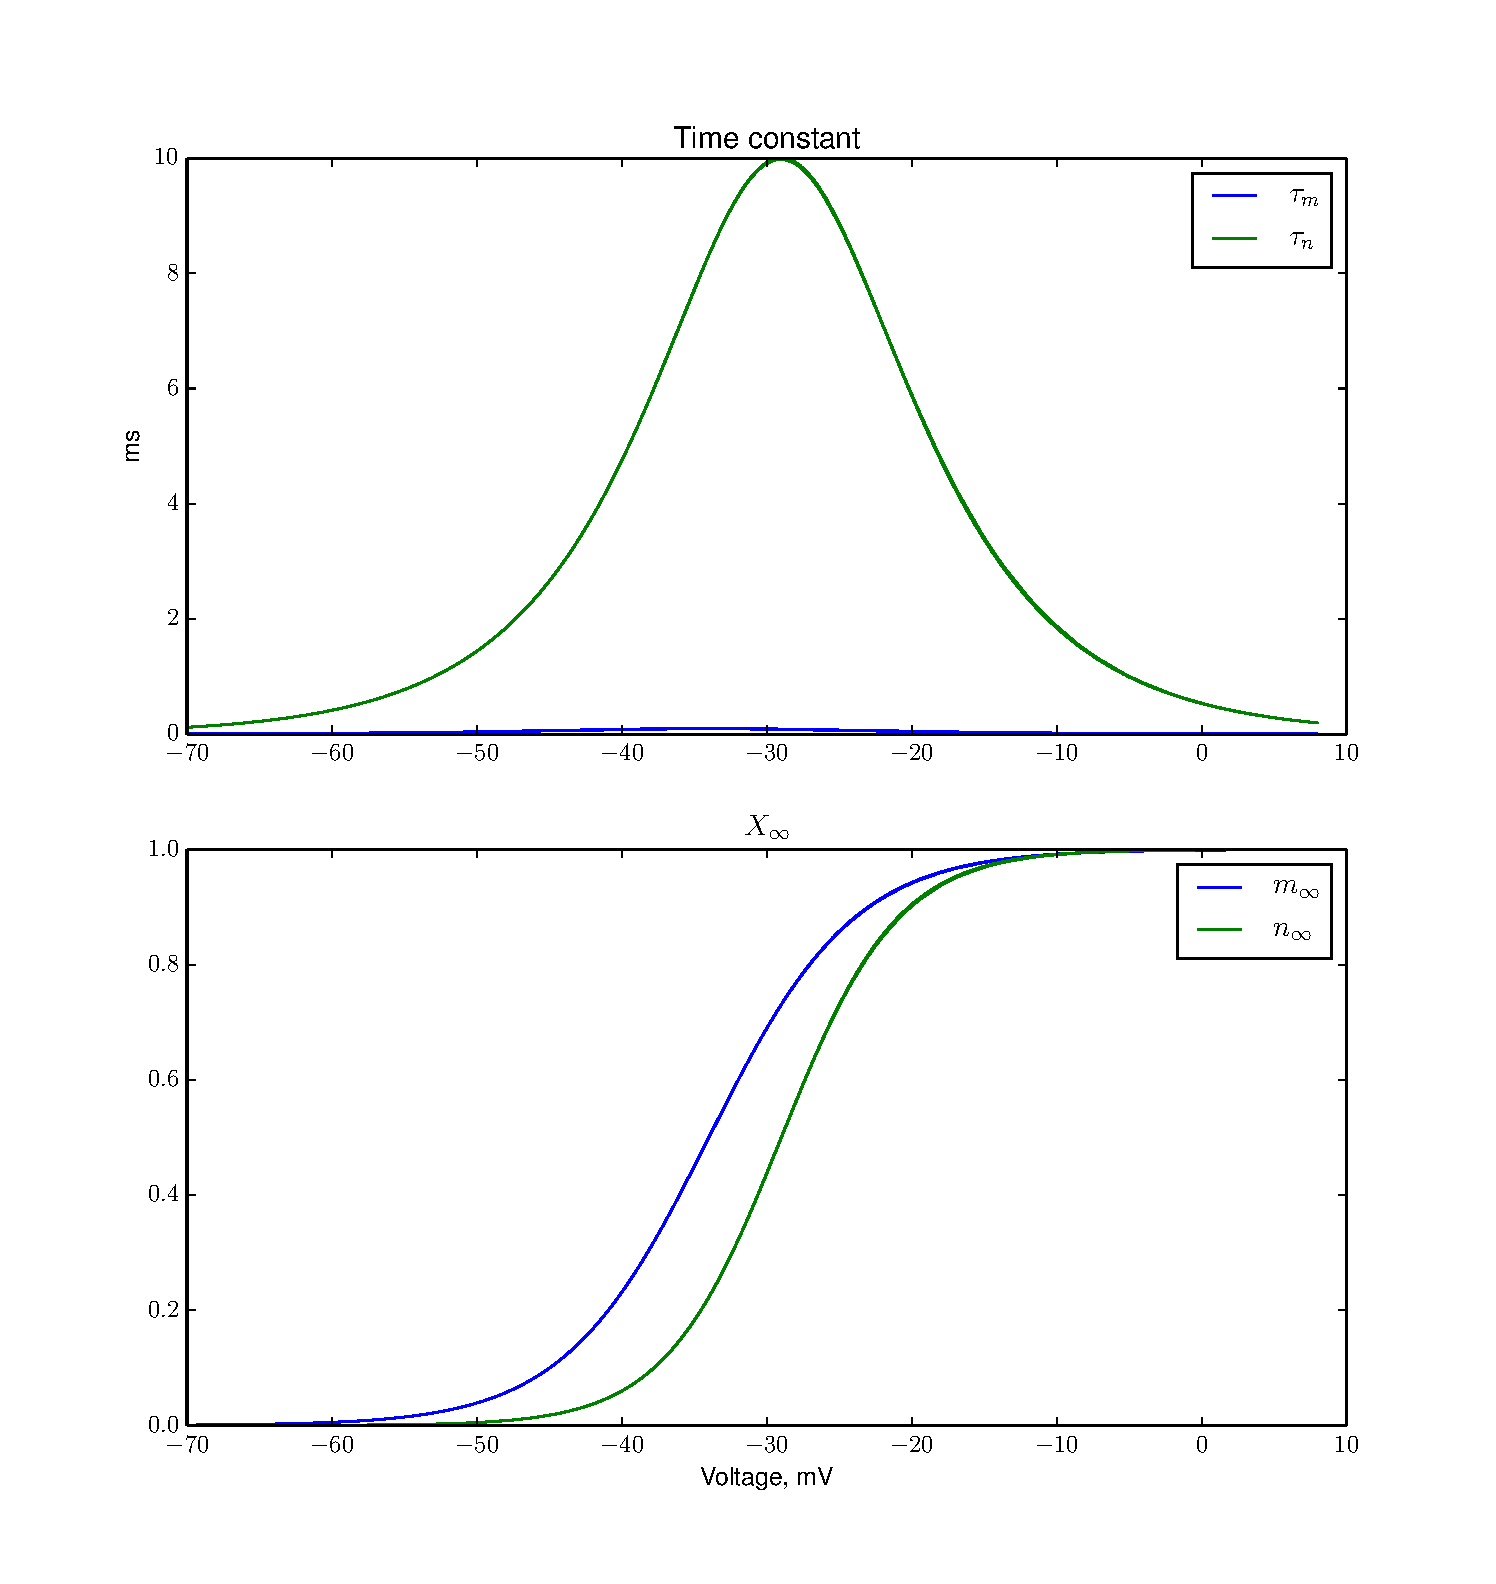
\includegraphics[width=\textwidth]{tau_inf}
    \caption{$\tau_\infty$}
    \label{fig:tau_inf}
\end{figure}

\section{Bursting neuron}
\subsection{Persistent sodium channel for repetitive firing}
\subsection{Slow potassium channel for bursting}
\section{Analysis of bursting and beating behaviors}
\subsection{Description of repetitive bursting}

\begin{figure}[H]
    \centering
    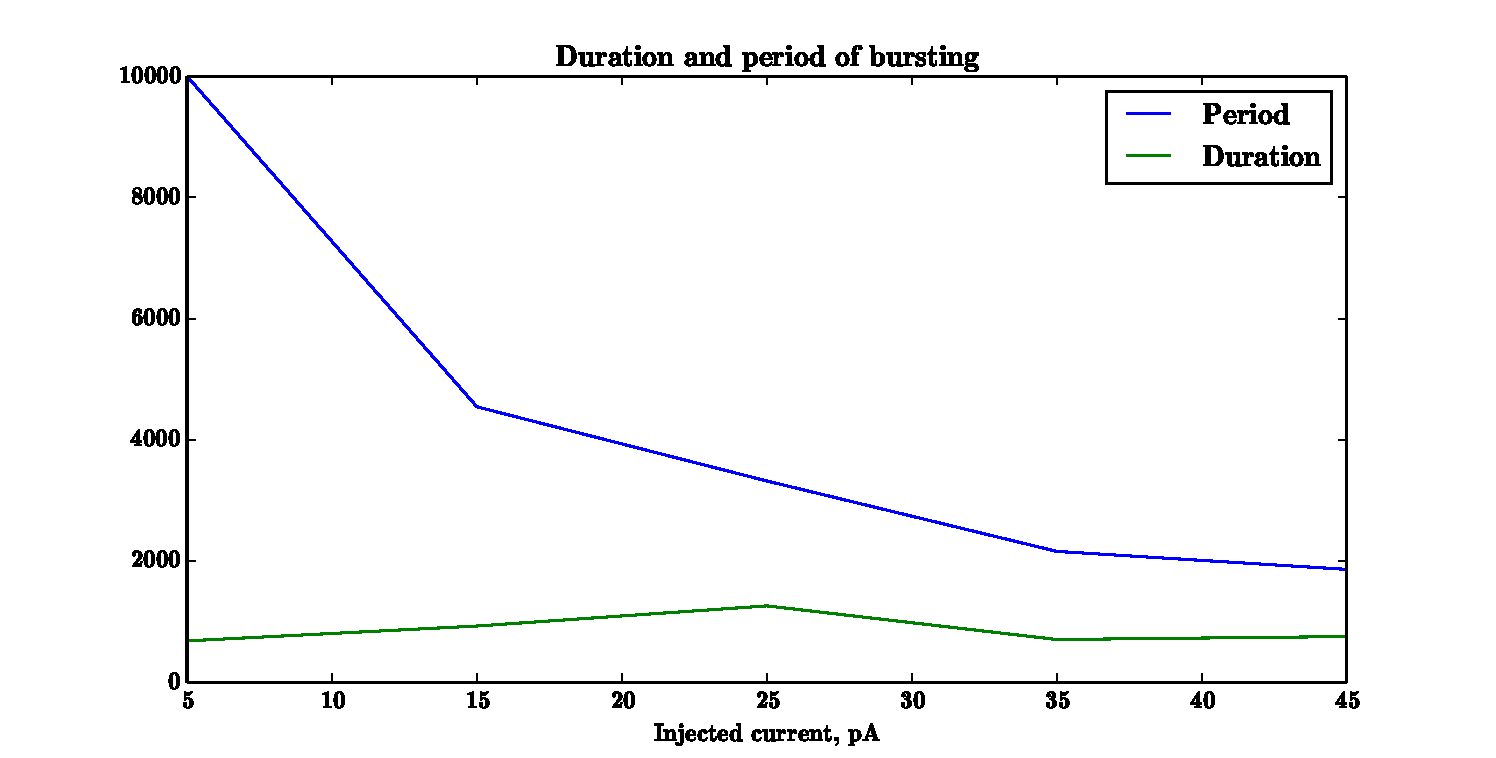
\includegraphics{bduration_bperiod}
    \caption{}
    \label{fig:bdur_bper}
\end{figure}

\subsection{Bursting and beating modes}
\subsection{Phase diagram}
\end{document}
